\documentclass[a4paper,11pt]{article}
\usepackage{graphicx}
\usepackage{enumerate}
\usepackage[usenames, dvipsnames]{color}

\begin{document}

\begin{flushright}

\vspace{1.1cm}

{\bf\Huge Apollo Guidance Computer}

\rule{0.25\linewidth}{0.5pt}
%\noindent\rule{\linewidth}{1.0pt}


\vspace{0.5cm}
%Put Authors
Justin Ely
\linebreak
\newline
%Put Author's affiliations
\footnotesize{605.411 Foundations of Computer Architecture \\}
\vspace{0.1cm}
% Date here below
6 December, 2016
\end{flushright}

\noindent\rule{\linewidth}{1.0pt}


%%%%%%%%%%%%%%%%%%%%%%%%%%%%%%%%%%%%%%%%%%%%%%%%%%%%%%%%%%

\section{Contents}
\begin{itemize}
\item Introduction %(page \pageref{sec:Introduction})
\item Data representation and Data Path
\item Instruction Set
\item Memory
\item Summary
\item References
\end{itemize}

%%%%%%%%%%%%%%%%%%%%%%%%%%%%%%%%%%%%%%%%%%%%%%%%%%%%%%%%%%

\section{Introduction and Overview}

While the Apollo project was beginning and taking shape in the 1960's, digital computing was still in it's infancy.  This provided great opportunities for the space program, from sharp decreases in size and sharp increases in power of computing equipement, but also caused a great deal of problems.  As history has shown, the pace of advancement in digital computing has been incredibly rapid, which can produce interesting results as both technology and mission requirements evolve over a decade of use.  

Both the Apollo Command Module and the Lunar Module employed a computer called the Apollo Guidance Computer (AGC) for control of guidance and navigation.  This included activities like changing velocity and orientation.  Astronauts would interface with the AGC through the Display and Keyboard interface (DSKY).  (MIT PDF)

\begin{figure}[h!]
\caption{Apollo Guidance Computer (AGC) {\it (left)} next to the DSKY (Display and Keyboard) interface {\it (right)}.} 
\centering
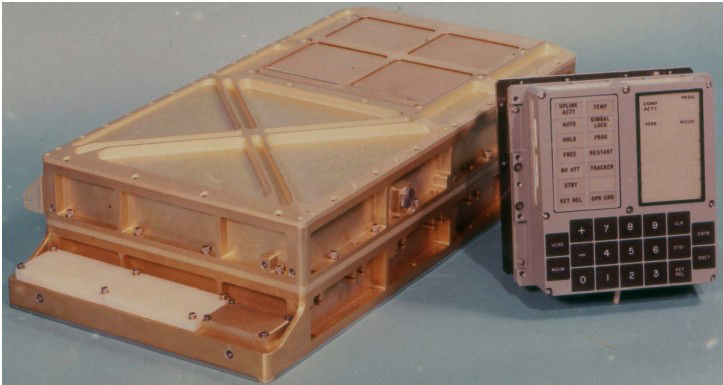
\includegraphics[width=.8\textwidth]{Agc_view.jpg} 
\end{figure}
\vspace{0.02cm}

Created by the Charles Stark Draper Laboratory and fabricated by Raytheon, the AGC was a modest 12.5x13x6 inches but weighed an impressive 70 pounds.  It used approx 55 watts of power which is comparable to a modern laptop.  (Wikipedia)

The APG utilized a Von Neumann Architecture with a CISC instruction set architecture.  The Von Neumann design, where both instructions and data occupied the same memory, served to simplify the hardware design and improve reliability. (MIT PDF).  The word size for the APG was 16 bits, with 1-bit dedicated to parity and not accessible to the programmer or user.  A total of 38K words of memory was available to the system.  The APG is also a One-address machine, which uses only a single register in instructions.  The other register is always assumed; typically the general-purpose accumulator the logical and arithmetic operations.  

Though the AGC represented some of the most cutting edge technology for the time, current technology highlights how far computing has gone in so little time.  By the 1980's, storage technology had advanced enough that the entirety of the command and lunar module software for all 6 lunar landings would easily fit on a single floppy disk.  Today, the entire APG memory system would fit into a modern CPU cache.

%%%%%%%%%%%%%%%%%%%%%%%%%%%%%%%%%%%%%%%%%%%%%%%%%%%%%%%%%%

\section{Data Representation and Data Path}
The data representation scheme used comes from the mission requirements to perform accurately evaluate equations for navigational computations.  This need for precise calculations was balanced against the waste that comes from too large of a word size.  Engineers determined that a word size of 16 bits (15 + 1 parity) was sufficient for instructions and gave enough precision for the mission.  This would allow two words to be read for 28 bits of precision (2 parity and 2 sign).  This gave approximated 8 decimals of precision and translated to distances of approx........ in the lunar missions.
The APG contained only integer arithmetic units.

Words were 16 bits (15 + 1 parity) for reasons that will be explained in later sections.  

\subsection{Integers}
The APG represents integers using a modified version of one's complement. As in the standard one's complement, 15 bits uses the first bit for the sign and the remaining 14 bits for the value.  This allows representation of values from -16383 to 16383 with both positive and negative zeros. Over flow is a problem with this scheme.

The modified scheme combats overflow by adding special detection of sign bit flips.  When doing calculations, the 15 bit value is loaded into a 16-bit accumulator, where the 16th bit is a copy of the sign bit from the operand.  This last bit is not accesible to the programmer; instead the AGC determines when an overflow occurs and alters programming accordingly.  

Namely, interrupts are temporarily prevented in the AGC (as the overflow detection bit would not be preserved accross an interrupt) until the overflow condition has been cleared.  Such as by loading a new value into the accumulator or clearing the content.  

Interestingly, when overflow does occur, the original sign bit (not the computed sign bit) is left in the register.  This keeps the value of the same sign, instead of opposite sign, but changes the actual magnitude.  

\subsection{Real Numbers}
With only integer units, the APG contained no units for representing, or performing arithmetic, on floating point numbers.   Instead, an alternative system was used to do calculations on real numbers.  This was called fractional notation.  

$\frac{1}{3} = .33331298828125$ in this fractional notation.  

Put burden on programmer to arrange programs to only need a single order of magnitude at a time so that only a fractional part (and not an exponent) is needed.

\subsection{Units}
Of interesting note is the mathematical units used in the computations.  Internally to the APG, the units were metric.  However, the astronauts wanted to read and input values in Imperial, so conversions were employed in the layer between the core and the UI.

%%%%%%%%%%%%%%%%%%%%%%%%%%%%%%%%%%%%%%%%%%%%%%%%%%%%%%%%%%

\section{Memory}
The memory system of the APG differs significantly from the systems we're used to today.  Physically, three different memory structures were employed; flip-flops for registers, coincident current ferrite cores for writable memory, and fixed core rope for read-only memory (ROM).  The use of magnetic memory was very important for space based applications as it was immune to most radiation-induced errors and would persist after the removal of the power source.

Ferrite-core?

magnetic core rope: The contents of read-only memory were physically written during fabrication.  This read-only memory held some programs, but also kept mathematical constants to prevent overwrite.  Ex. star locations, etc.  This memory was compact, reliable, had random access, and was extremely inexpensive.  Each bit cost between \$.05 and \$.07 to produce when most comparable solutions were a factor of 10 higher. (MIT) The main detractor to rope memory came from it's characteristic of being programmed during production.  This meant that any desired change, due to changing requirements or simple mistakes in programming or manufacture, couldn't be implemented without re-wiring the core.  Due to their complexity, this usually meant entire modules needed to be replaced for any change.  (MIT)

Of the 38K words in total system memory, the first 48 words belonged to the central registers.  (FIXME, Explain the various ones?)  The next 2K were the writable memory, and the remaining 36K were ROM.  Furthering the departments from current trends, the registers were addressable just like the other memory locations.  This allows the same instructions to be used for memory and register access.  

It may have been apparent that the 12-bit addresses in the instruction set can only reference 4K of storage and are not sufficient to address all locations in the 38K memory space.  At this time in history, memory was relatively cheap and allowed systems to have far more memory than was physically addressable with a reasonable word-size.  Contrast this today, where modern 64-bit word-sizes can address far more memory than can be included with the system.  
Virtual memory management wasn't yet in a mature form at this time in computing history. 

To combat this, a "memory banking" scheme was used. Bank registers.

%%%%%%%%%%%%%%%%%%%%%%%%%%%%%%%%%%%%%%%%%%%%%%%%%%%%%%%%%%

\section{Instruction Set}
The APG is a Complex Instruction Set Computer (CISC), where instructions perform complex tasks through microprogrammed implementations requiring many clock cycles.  This is clearly evident in many of the available commands, such as ADS which performs addition into a memory location.  This behavior is in stark contrast to a Reduced Instruction Set Computer (RISC), where typically only Load and Store commands may access memory.  

The basic format for instructions in the AGC is shown below.  The first bit provides parity, the next 3 bits are the op-code, and the remainder is the address.  

\begin{center}
\begin{tabular}{| c | c | c |}
  \hline	
  	Parity & Op-code & Address \\ \hline \hline
	1 & 011 & 000110101110 \\ \hline
\end{tabular} \\
\end{center}

A 3-bit opcode allows for a total of 8 unique instructions.  Clearly, trying to work the entire operation of a complicated spacecraft with only 8 instructions would present significant challenges.  More instructions were necessary, but even as the mission requirements progressed it would be too costly to re-design the system around a larger word size.  The engineers created some unique solutions to get more instructions within the existing limitations.

The first addition to the instruction set came from exploiting existing commands that could utilize smaller operand fields.  In particular, instructions that write to memory don't need to access the higher addresses of the ROM, and will only ever use the lower 10 bits of the operand field. By combining the two left-over bits, called quarter-codes, with the opcodes for this subset of commands yields an entirely new suite of available instructions.  

The quarter codes expanded the instruction set considerably, and added efficiency to the system by giving useful meaning to commands and addresses that wouldn't work with the memory system, but still more were needed.  To further add to the available commands, the engineers repurposed nonsensical (though valid) instructions.  One example of this would be using the TC command to transfer control to the EBANK register.  This register was only 3 bits wide and would never contain valid instructions or data.  Instead, the AGC turned TC to EBANK into a brand new instruction: RELINT (Enable Interrupts).  Similarly, this was done for TC commands to 3 other registers that would never be valid.  This strategy served not only to expand the available commands, but to also serve as protection against programmer error.  If TC to EBANK ever was accidently entered, without the protection of the special commanding, the effects could be very difficult to debug.

Similarly, a 12-bit address also presents a problem.  12 bits is sufficient only to address 4K of memory; far short of the 38K necessary. 

\subsection{Quarter-codes, special cases, extend}
quarter codes: commands that modify writable memory (TS, ADS, INCR, XCH) all need to have 0's in bits 11 and 12. 

op-code 000 links to many special instructions (I/O)

op-code 011, 100, 111 are all single instructions. 
The four remaining binary opcodes
(001, 010, 101 and 110) use quarter codes to varying degree

Special cases:  Pg 84.  Used invalid TC commands as entirely new commands.

EXTEND set

\begin{center}
\begin{tabular}{| c | c | c |}
  \hline	
  	Group & Command & Meaning \\ \hline \hline
	Sequence Changing & TC & Transfer Control \\ \hline
	& TCF & Transfer Control to Fixed \\ \hline
	& CCS & Count Compare and Skip \\ \hline
	& BZF & Branch Zero to Fixed \\ \hline
	& BZMF & Branch Zero or Minus to Fixed \\ \hline
	
	Reading and Writing & CA & Clear and Add \\ \hline
	& CS & Clear and Subtract \\ \hline
	& DCA & Double Clear and Add \\ \hline
	& DCS & Double Clear and Subtract \\ \hline
	& TS & Transfer to Storage \\ \hline
	& XCH & Exchange A and K \\ \hline
	& LXCH & Exchange L and K \\ \hline
	& QXCH & Exchange Q and K \\ \hline
	& DXCH & Double Exchange \\ \hline
	
	Instruction Modification & INDEX & Index Next Instruction \\ \hline
	& INDEXE & Index Next Instruction Extended \\ \hline
	
	Arithmetic and Logic & AD & Add \\ \hline
	& Su & Subtract \\ \hline
	& ADS & Add to Storage \\ \hline
	& MSU & Modular Subtract \\ \hline
	& INCR & Increment \\ \hline
	& AUG & Augment \\ \hline
	& DIM & Diminish \\ \hline
	& DAS & Double Add to Storage \\ \hline
	& MASK & Mask A by K \\ \hline
	& MP & Multiply \\ \hline
	& DV & Divide \\ \hline

	I/O Channel & READ & READ KC \\ \hline
	& WRITE & Write Channel KC \\ \hline
	& RAND & Read and Mask \\ \hline
	& WAND & Write and Mask \\ \hline
	& ROR & Read and Superimpose \\ \hline
	& WOR & Write and Superimpose \\ \hline
	& RXOR & Read and Invert \\ \hline

	Miscellaneous & XXALQ & Execute Extracode Using A, L, and Q \\ \hline
	& XLQ & Execute Using L and Q \\ \hline
	& RETURN & Return From Subroutine \\ \hline
	& RELINT & Enable Interrupts \\ \hline
	& INHINT & Inhibit Interrupts \\ \hline
	& EXTEND & Set Extracode Flag \\ \hline
	& EDRUPT & Ed Smally's Interrupt \\ \hline	
	& RESUME & Resume Interrupted Program \\ \hline	


	Involuntary & RUPT & Interrupt \\ \hline
	& PINC & Counter Increment \\ \hline
	& MINC & Counter Decrement \\ \hline
	& DINC & Diminish Absolute Value by 1 \\ \hline
	& PCDU & CDU Increment \\ \hline
	& MCDU & CDU Decrement \\ \hline
	& SHINC & Counter Shift \\ \hline
	& SHANC & Counter Shift and Add 1 \\ \hline
	
\end{tabular} \\
\end{center}

%%%%%%%%%%%%%%%%%%%%%%%%%%%%%%%%%%%%%%%%%%%%%%%%%%%%%%%%%%

\section{Summary}


%%%%%%%%%%%%%%%%%%%%%%%%%%%%%%%%%%%%%%%%%%%%%%%%%%%%%%%%%%

\section{References}

\begin{itemize}
  \item The Apollo Guidance Computer: architecture and operation, Frank O'Brien., Chichester : Praxis, 2010.
  \item https://en.wikipedia.org/wiki/Apollo\_Guidance\_Computer
  \item Apollo 11 Guidance Computer source code: https://github.com/chrislgarry/Apollo-11/
  \item Delco Electronics, Apollo 15 - Manual for CSM and LEM AGC software used on the Apollo 15 mission
\end{itemize}

\end{document}
